%%
%% Cover Letter — Biodiversity and Conservation (Springer Nature)
%%
\documentclass[12pt]{article}
\usepackage[T1]{fontenc}
\usepackage[utf8]{inputenc}
\usepackage[american]{babel}
\usepackage[margin=2.5cm]{geometry}
\usepackage{setspace}
\onehalfspacing
\usepackage{hyperref}
\usepackage{graphicx}
\graphicspath{{../../../3-FIGURAS/}}

\pagestyle{empty}

\begin{document}

\noindent
\begin{minipage}[c]{0.15\textwidth}
\centering

\includegraphics[height=1.5cm]{logo_uefs.png}
\end{minipage}%
\hfill
\begin{minipage}[c]{0.60\textwidth}
\centering
{\large\bfseries Universidade Estadual de Feira de Santana -- UEFS}\\[4pt]
Departamento de Ci\^encias Humanas e Filosofia -- DCHF\\[4pt]
Programa de Pós Graduação em Planejamento Territorial -- Planter
\end{minipage}%
\hfill
\begin{minipage}[c]{0.20\textwidth}
\centering
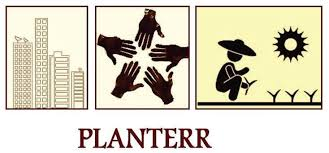
\includegraphics[height=1.5cm]{logo_planter.jpg}
\end{minipage}

\vspace{12pt}

\noindent
Cover Letter\\
\textit{Biodiversity and Conservation}\\
Springer Nature

\vspace{18pt}

\noindent
On behalf of all co-authors, I am pleased to submit the manuscript entitled ``Institutional fragility and climatic exposure drive biocultural vulnerability in traditional agricultural knowledge systems'' for possible publication in the journal \textit{Biodiversity and Conservation}.

\vspace{6pt}

\noindent
This work presents the first hierarchical meta-analysis quantifying how eight dimensions of biocultural vulnerability are associated with the degradation of Traditional Agricultural Knowledge Systems (TAKS). By integrating a systematic review (2016--2026) of 47 studies comprising 363 observations with a three-level mixed-effects model and robust variance estimation, we identify legal and land tenure vulnerability as the greatest degradation driver, with a 24.3\% erosion in formal protection indicators, and climatic exposure as the second significant effect, corresponding to a 32.3\% increase in vulnerability indicators associated with extreme events. The meta-regression reveals that South American farming communities concentrate the greatest legal fragility (37.1\% erosion), whereas interventions anchored in symbolic territories---such as sacred groves---yield the highest protective effects on both social organization and linguistic vitality. The study provides an original contribution by offering the first quantitative synthesis that links institutional fragility, climatic exposure, and community-level moderators to the vulnerability of traditional knowledge systems, delivering actionable evidence for heritage conservation policies in biodiversity-rich regions. This extends the scientific understanding of biocultural diversity loss and safeguarding mechanisms.

\vspace{6pt}

\noindent
The manuscript represents original and unpublished research that has not been submitted elsewhere. All authors have approved the final version and consent to its submission. The systematic review protocol is registered on the Open Science Framework (DOI: 10.17605/OSF.IO/HE8KT), and the extraction dataset, analysis scripts, and meta-analytic outputs are deposited on Mendeley Data (DOI: 10.17632/mh5sbx7ky7.1), ensuring full transparency and replicability. We believe that this study aligns strongly with the journal's scope on conservation science that integrates biological and cultural dimensions of diversity.

\vspace{6pt}

\noindent
We kindly appreciate your consideration and look forward to your feedback.

\vspace{36pt}

\noindent
Sincerely,

\vspace{36pt}

\noindent
Luiz Diego Vidal Santos, PhD\\
(Corresponding Author)\\
Universidade Estadual de Feira de Santana (UEFS)\\
E-mail: ldvsantos@uefs.br

\end{document}
